% ============================================================================
% Periodic Poisson problem: direct, AMG, static-condensation and spectral solvers
% Generated by tools/periodic_poisson_benchmark/latex.py from results.csv
% (Jexpresso branch sm/elementLearning). Do not edit the numbers by hand:
% re-run the benchmark and this script.
% Needs: \usepackage{amsmath,amssymb,booktabs,pgfplots} \pgfplotsset{compat=1.17}
% ============================================================================
\definecolor{jxsem}{RGB}{42,120,214}
\definecolor{jxsemamg}{RGB}{235,104,52}
\definecolor{jxscdirect}{RGB}{27,175,122}
\definecolor{jxscamg}{RGB}{237,161,0}
\definecolor{jxps}{RGB}{232,123,164}
\definecolor{jxfft}{RGB}{0,131,0}
\section{Linear solvers for the spectral-element Poisson problem: direct, algebraic multigrid, static condensation and spectral baselines}
\label{sec:solver-comparison}

This section compares the solvers available in Jexpresso for the linear system
of a steady, doubly periodic Poisson problem: the sparse direct solve and an
algebraic-multigrid (AMG) solve of the full spectral-element (SEM) system, the
same two solves applied after static condensation --- the reduction on which
element learning is built --- and two global spectral baselines, a
pseudo-spectral Fourier collocation method and an FFT solver.

\subsection{Test problem and discretisations}
\label{sec:sc-problem}
We solve
\begin{equation}
  -\nabla^2 u = f \quad\text{on } \Omega=[0,2\pi]^2,\qquad u \text{ periodic in } x \text{ and } y,
  \label{eq:sc-poisson}
\end{equation}
with the manufactured solution
\begin{equation}
  \begin{gathered}
  u(x,y)=A\Big(p(x)\,p(y)-\frac{1}{c^2-1}\Big),\qquad p(s)=\frac{1}{c-\cos s},\\
  f=-\nabla^2u=-A\big(p''(x)\,p(y)+p(x)\,p''(y)\big),
  \end{gathered}
  \label{eq:sc-exact}
\end{equation}
where $p''(s)=-\cos s/(c-\cos s)^2+2\sin^2 s/(c-\cos s)^3$, $c=(r+r^{-1})/2$ with
$r=0.8$, and $A=(c-1)^2(c+1)/2$ scales the peak to $u(0,0)=1$. The periodic Poisson
kernel $p$ has the Fourier series
$p(s)=(c^2-1)^{-1/2}\big(1+2\sum_{k\ge1}r^k\cos ks\big)$. The Fourier coefficients of $u$
therefore decay geometrically, like $r^{|k_x|+|k_y|}$, and $u$ is not band-limited: a
Fourier method on an $N_g\times N_g$ grid has a grid-dependent error, about
$r^{N_g/2}$, as does the SEM. Since the mean of $p$ is $(c^2-1)^{-1/2}$, $u$ has zero
mean, and so does $f$ (the integral of a Laplacian over a period). $u$ is therefore
the zero-mean solution of \eqref{eq:sc-poisson}, which is the one every solver
returns (the constants span the null space of the periodic Laplacian).

\paragraph{SEM.} The mesh has $16\times16$ quadrilateral elements of polynomial order
$N=2,\dots,8$ on the Legendre--Gauss--Lobatto nodes, i.e.\ $n=(16N)^2$
unknowns after periodic identification. Periodicity enters the continuous-Galerkin
system by giving the two copies of a seam node the same global number; the
stiffness matrix $K$ is assembled on the periodic unknowns and the load is
$\mathbf b=M\mathbf f$ with the lumped mass matrix $M$. $K$ is symmetric positive
semi-definite with $K\mathbf 1=\mathbf 0$: the mean of $\mathbf b$ is projected out
(compatibility), one unknown is pinned, and the solution is shifted to zero
$M$-weighted mean.

\paragraph{Fourier solvers.} The pseudo-spectral and FFT solvers work on a uniform
$16N\times16N$ grid, i.e.\ with the same number of unknowns as the SEM of
order $N$. The pseudo-spectral solver is Fourier collocation with Kopriva's
derivative matrix $D$; the second derivative $D\cdot D$ is corrected on the Nyquist
mode (which $D$ annihilates for an even number of points) so that it equals the
Fourier second-derivative collocation matrix $D^{(2)}$, and the tensor-product
system is solved by matrix diagonalisation, $O(N^3)$ operations per solve. The FFT
solver divides the real FFT of $f$ by $|\mathbf k|^2$ (FFTW), $O(N^2\log N)$
operations per solve.

\subsection{Static condensation}
\label{sec:sc-method}
Split the unknowns into the element interiors $o$ (the $(N-1)^2$ nodes strictly
inside each element) and the element skeleton $b$ (the nodes on element edges).
Every interior node belongs to one element, so $A_{oo}$ is block diagonal, and
eliminating the interiors gives the Schur-complement (skeleton) system
\begin{equation}
  B\,\mathbf u_b=\hat{\mathbf f}_b,\qquad
  B = A_{bb}-\sum_{e}A_{b,o_e}T^{e},\qquad
  \hat{\mathbf f}_b=\mathbf f_b-\sum_e A_{b,o_e}\,\mathbf t^{e},
  \label{eq:sc-schur}
\end{equation}
with the local operators
\begin{equation}
  T^{e}=A_{o_eo_e}^{-1}A_{o_eb_e},\qquad \mathbf t^{e}=A_{o_eo_e}^{-1}\mathbf f_{o_e},
  \label{eq:sc-local}
\end{equation}
followed by the element-by-element recovery $\mathbf u_{o_e}=\mathbf t^e-T^e\mathbf u_{b_e}$.
This is the algorithm of element learning, which replaces $T^e$ by the output of a
trained network. Here $T^e$ is computed from the element blocks of the SEM matrix, so
the condensation is an exact algebraic reduction that reproduces the full SEM
solution to round-off. In the periodic problem there is no Dirichlet boundary, the
skeleton system is singular like $K$, and it is gauged in the same way. The skeleton
has $16^2(2N-1)$ unknowns: $3\,840$ of the $16\,384$ unknowns at
$N=8$.

\begingroup\sloppy
\subsection{Common SEM infrastructure}
\label{sec:alg-sem-common}
The four SEM solvers share one discretisation, built by the driver before the linear
solve (\texttt{sem\_setup}). This subsection describes that code path and the reduction
to the periodic system that all four solve.

\paragraph{Mesh.} The deck reads a Gmsh mesh of $16\times16$ straight-sided
quadrilaterals on $[0,1]^2$ whose boundary edges are tagged periodic in $x$ and in $y$.
With refinement level $L>0$ (\texttt{:linitial\_refine}, \texttt{:init\_refine\_lvl}$\,=L$)
the mesh is refined uniformly $L$ times by p4est
(\texttt{UniformlyRefinedForestOfOctreesDiscreteModel}), giving $n_e\times n_e$ elements
with $n_e=16\cdot2^L$. The high-order nodes are added on the edges and in the
interiors. The node coordinates are then mapped by
$x\leftarrow(x+x_{\rm disp})\,x_{\rm scale}/2$ with $x_{\rm disp}=0$, $x_{\rm scale}=4\pi$,
and likewise in $y$, which gives $[0,2\pi]^2$. The local node numbering is not merged
across the periodic seams. Instead, the periodic restructuring gives the two (or four,
at a corner) local copies of a seam node the same global number in
\texttt{mesh.ip2gip}.

\paragraph{Basis and quadrature.} The $N+1$ Legendre--Gauss--Lobatto (LGL) nodes
$\xi_k$ and weights $\omega_k$ come from Kopriva's algorithm: Newton iteration on
$q=L_{N+1}-L_{N-1}$ from the Chebyshev-like initial guess
$-\cos\big((j+\tfrac14)\pi/N-3/(8N\pi(j+\tfrac14))\big)$, with tolerance $4\varepsilon$ and
$\omega_j=2/\big(N(N+1)L_N(\xi_j)^2\big)$. The quadrature is \emph{inexact}: it uses the
same $N+1$ LGL points ($Q=N$), which is the default \texttt{:lexact\_integration =>
false}. The 1-D Lagrange basis $\psi_i$ and its derivative $\psi_i'$ are evaluated at the
quadrature points with the product formula (Giraldo, Algorithms 3.1--3.2). Because the
interpolation and quadrature points coincide, $\psi_i(\xi_k)=\delta_{ik}$.

\paragraph{Metric terms.} For each element and quadrature point $(k,l)$:
$x_\xi=\sum_{i,j}\psi_i'(\xi_k)\psi_j(\xi_l)\,x_{ij}$ and $x_\eta=\sum_{i,j}\psi_i(\xi_k)\psi_j'(\xi_l)\,x_{ij}$
(likewise $y_\xi,y_\eta$), $J=x_\xi y_\eta-y_\xi x_\eta$, and
$\xi_x=y_\eta/J$, $\xi_y=-x_\eta/J$, $\eta_x=-y_\xi/J$, $\eta_y=x_\xi/J$
(\texttt{build\_metric\_terms!}).

\paragraph{Element Laplacian.} With $\Psi_{mn}(\xi,\eta)=\psi_m(\xi)\psi_n(\eta)$ and
\[
  \partial_x\Psi_{mn}\big|_{kl}=\psi_m'(\xi_k)\psi_n(\xi_l)\,\xi_x+\psi_m(\xi_k)\psi_n'(\xi_l)\,\eta_x
\]
(likewise $\partial_y$), the element stiffness matrix is
\begin{equation}
  L^e_{mn,ij}=\sum_{k,l=1}^{N+1}\omega_k\omega_l\,J_{kl}\,
  \big(\partial_x\Psi_{mn}\,\partial_x\Psi_{ij}+\partial_y\Psi_{mn}\,\partial_y\Psi_{ij}\big)\big|_{kl},
  \label{eq:alg-Le}
\end{equation}
the positive semi-definite form of $-\nabla^2$ (\texttt{build\_laplace\_matrix}). It is
stored densely for every element, $n_e^2(N+1)^4$ numbers.

\paragraph{Assembly.} The global matrix $L$ is assembled on the \emph{local} nodes
(\texttt{DSS\_laplace\_sparse}). For every element and every pair of its nodes, the
triplet $(\text{row}, \text{column}, L^e)$ is recorded, but only when
$|L^e|>\varepsilon=2.2\times10^{-16}$. One call to \texttt{sparse} then sums the
duplicate entries. Because the seam copies are distinct local nodes, $L$ is the
stiffness matrix of the box with natural boundaries: the copies are not yet coupled.

\paragraph{Mass matrix.} The element mass matrix
$M^e_{IJ}=\sum_{k,l}\omega_k\omega_lJ_{kl}\Psi_I\Psi_J|_{kl}$ is diagonal, because
$\psi_i(\xi_k)=\delta_{ik}$. Its rows are summed into a vector $M$ on the local nodes
(\texttt{DSS\_mass!}). The global DSS (\texttt{DSS\_global\_mass!}, through
\texttt{assemble\_mpi!}) then sums the entries of all local nodes that share a global
number. Every seam copy therefore holds the mass of its whole periodic class.

\paragraph{Periodic system} (\texttt{periodic\_sem\_system}). The local nodes are grouped
into classes $c=1,\dots,m$ by their global number (\texttt{unique(ip2gip)}). The
representative $r_c$ of a class is its lowest local index, and $P$ is the
$n_{\rm loc}\times m$ incidence matrix, $P_{i,c(i)}=1$. Then
\begin{equation}
  K=P^{\mathsf T}(LP),\qquad w_c=M_{r_c},\qquad b_c=M_{r_c}\,f(\mathbf x_{r_c}),
  \label{eq:alg-K}
\end{equation}
with $f$ evaluated at every local node by the case's \texttt{user\_source!}.
$K$ has $m=(n_eN)^2$ rows, is exactly symmetric, and satisfies $K\mathbf 1=0$. The
right-hand side is projected onto the range of $K$:
$\bar f=\sum_cb_c/\sum_cw_c$ and $\mathbf b\leftarrow\mathbf b-\bar f\,\mathbf w$.
All four SEM solvers solve $K\mathbf u=\mathbf b$ with the same gauge: the first
class is pinned, $u_1=0$, and afterwards $\mathbf u\leftarrow\mathbf u-(\mathbf w^{\mathsf T}\mathbf u)/(\mathbf w^{\mathsf T}\mathbf 1)$.
The solution of each class is copied to all its local nodes.

\subsection{Algorithm: SEM direct}
\label{sec:alg-sem-direct}
\begin{enumerate}
  \item \emph{Setup} (\texttt{periodic\_sem\_factorize}): \texttt{F = factorize(K[2:end,2:end])}.
        Julia's \texttt{factorize} tests the matrix; $K$ is exactly symmetric, so it
        returns a CHOLMOD sparse Cholesky factor (SuiteSparse), with CHOLMOD's own
        fill-reducing ordering (symbolic analysis plus numeric factorisation).
  \item \emph{Solve} (\texttt{periodic\_sem\_direct\_solve}): $u_1=0$,
        $\mathbf u_{2:m}=F\backslash\mathbf b_{2:m}$ (forward and backward triangular
        solves), then the $\mathbf w$-weighted gauge.
\end{enumerate}
The setup time also includes the periodic reduction \eqref{eq:alg-K}.

\subsection{Algorithm: SEM AMG}
\label{sec:alg-sem-amg}
\begin{enumerate}
  \item \emph{Setup} (\texttt{jx\_amg\_setup}): $K_{2:m,2:m}$ is converted to
        \texttt{SparseMatrixCSC\{Float64,Int\}}, and \texttt{smoothed\_aggregation} of
        AlgebraicMultigrid.jl builds the hierarchy with the package defaults:
        \begin{itemize}
          \item symmetric strength of connection with $\theta=0$;
          \item standard aggregation;
          \item tentative prolongator from the constant near-null-space vector, improved by
                four symmetric Gauss--Seidel iterations and smoothed by weighted Jacobi
                with $\omega=4/3$;
          \item at most 10 levels; coarsening stops at 10 unknowns, and the coarsest
                system is solved with a dense pseudo-inverse.
        \end{itemize}
        \texttt{aspreconditioner} wraps it: one application is one V-cycle from a
        zero initial guess, with one symmetric Gauss--Seidel sweep before and one after
        each coarse-grid correction.
  \item \emph{Solve} (\texttt{jx\_amg\_solve}): \texttt{Krylov.cg} with this
        preconditioner (\texttt{ldiv=true}), from $\mathbf x_0=0$, $u_1=0$, and then
        the $\mathbf w$-weighted gauge. CG stops when the preconditioned residual
        norm $\sqrt{\mathbf r^{\mathsf T}M^{-1}\mathbf r}$ falls below
        $10^{-12}$ times its initial value (\texttt{rtol}; \texttt{atol}$\,=0$), or
        after \texttt{:amg\_itmax} iterations (10\,000 in the benchmark).
\end{enumerate}

\subsection{Algorithm: SC direct}
\label{sec:alg-sc-direct}
The static condensation of Section~\ref{sec:sc-method} is applied to $K\mathbf u=\mathbf b$
by the element-learning routine \texttt{elementLearning\_Axb!}, with the local
operators computed from $K$ (no network). The set-up is done in
\texttt{periodic\_sem\_sc\_solve}:
\begin{enumerate}
  \item \emph{Class-numbered mesh.} Each element's node list \texttt{mesh.conn} lists
        its $4N$ boundary nodes first and its $(N-1)^2$ interior nodes last; it is
        rewritten in class numbers. The skeleton $\partial O$ is the sorted set of
        classes of the boundary nodes, and $I_o$ is the set of classes of the
        interior nodes. The code checks that every interior class belongs to one
        element only and not to the skeleton, and that
        $|\partial O|+|I_o|=m$. There is no Dirichlet set ($\Gamma=\emptyset$),
        so $\partial\tau=\partial O$, and $|\partial O|=n_e^2(2N-1)$.
  \item \emph{Extraction.} The sparse blocks $K_{\partial\tau\partial\tau}$ and
        $K_{\partial O\partial\tau}$ are sliced from $K$. For every element, the dense
        blocks $A^e_{oo}$ ($(N-1)^2\times(N-1)^2$), $A^e_{ob}$ ($(N-1)^2\times4N$) and
        $A^e_{bo}$ ($4N\times(N-1)^2$) are read entry by entry from $K$, and the
        interior load $\mathbf f^e_o=\mathbf b[I_o^e]$ is taken from the projected
        right-hand side.
  \item \emph{Condensation.} For every element the dense inverse
        $(A^e_{oo})^{-1}$ is formed explicitly (\texttt{inv}, LAPACK), and then
        $T^e=(A^e_{oo})^{-1}A^e_{ob}$ and $\mathbf t^e=(A^e_{oo})^{-1}\mathbf f^e_o$.
        Each entry of $A^e_{bo}T^e$ whose row is in $\partial O$ and column in
        $\partial\tau$ is recorded as a triplet, and
        $\Delta\mathbf f\mathrel{+}=A^e_{bo}\mathbf t^e$ is accumulated. After the
        element loop, \texttt{sparse} sums the triplets into $\Delta B$, and
        \begin{equation}
          B=K_{\partial O\partial\tau}-\Delta B,\qquad
          \hat{\mathbf f}=\mathbf b_{\partial O}-\Delta\mathbf f\quad(-\,B_{\partial O\Gamma}\mathbf g_\Gamma=0\text{ here}).
        \end{equation}
  \item \emph{Skeleton solve} (\texttt{el\_skeleton\_solve}, with
        \texttt{singular = true} because $\Gamma=\emptyset$): the first skeleton
        unknown is pinned. $B$ is symmetric in exact arithmetic, but the subtraction
        leaves a round-off asymmetry ($\approx10^{-16}$ relative), enough for
        \texttt{factorize}, which tests for exact symmetry, to fall back to LU. The
        code therefore symmetrises the pinned matrix, $\tfrac12(B+B^{\mathsf T})$,
        which is bitwise symmetric because floating-point addition commutes. It warns
        if the relative asymmetry exceeds $10^{-10}$, which would not be round-off. It
        then factorises the result with CHOLMOD sparse Cholesky
        (\texttt{cholesky}), as for the full system, and solves with
        \texttt{F \textbackslash{} rhs}. LU is used only if $B$ is not positive
        definite, and then with a warning.
  \item \emph{Interior recovery.} For every element,
        $\mathbf r^e=\mathbf f^e_o-A^e_{o\,\partial O}\mathbf u_{\partial O}$, the
        inverse of $A^e_{oo}$ is formed again (\texttt{inv}), and
        $\mathbf u_{o}^e=(A^e_{oo})^{-1}\mathbf r^e$.
  \item The $\mathbf w$-weighted gauge is applied to the full class vector.
\end{enumerate}
Timing: the setup is the periodic reduction plus steps 1--3 plus the factorisation
in step 4. The solve step is the triangular solves in step 4 plus step 5.

\subsection{Algorithm: SC AMG}
\label{sec:alg-sc-amg}
Identical to SC direct except in step 4, where the pinned skeleton matrix
$B_{2:,2:}$ goes through \texttt{jx\_amg\_setup} and \texttt{jx\_amg\_solve}. These
use the same smoothed-aggregation hierarchy and CG settings as SEM AMG
(Section~\ref{sec:alg-sem-amg}): relative tolerance $10^{-12}$ on the preconditioned
residual norm. The setup contains the AMG hierarchy of $B$, and the solve step
contains the CG iterations and the interior recovery.

\subsection{Algorithm: pseudo-spectral (Fourier collocation)}
\label{sec:alg-ps}
The pseudo-spectral and FFT solvers do not use the SEM mesh: the driver dispatches
to them before \texttt{sem\_setup}. Both use the uniform periodic grid
$x_i=iL_x/N_g$, $y_j=jL_y/N_g$, $i,j=0,\dots,N_g-1$ (the right-hand periodic image
is not stored), with $N_g=n_eN$ (\texttt{:fft\_N}) and $L_x=L_y=2\pi$.
\begin{enumerate}
  \item \emph{Right-hand side:} $F_{ij}=f(x_i,y_j)$ is sampled on the grid.
  \item \emph{Setup, per axis} (\texttt{\_collocation\_axis}): Kopriva's Fourier
        derivative matrix for even $N_g$ (Algorithm~18) has
        $D_{ij}=\tfrac12(-1)^{i+j}\cot\big((i-j)\pi/N_g\big)$ for $i\neq j$, and
        $D_{ii}=-\sum_{j\neq i}D_{ij}$; it is scaled by $2\pi/L$. Form
        $A=-D\,D$ and compute the symmetric eigendecomposition of
        $(A+A^{\mathsf T})/2$ (\texttt{eigen(Symmetric(\dots))}, LAPACK). The code
        requires exactly two eigenvalues with $|\lambda|<10^{-6}(2\pi/L)^2$; $D\,D$
        annihilates both the constant and the Nyquist mode $\cos(N_gx/2)$. Their
        eigenvectors are replaced by the exact vectors $1/\sqrt{N_g}$ and
        $(-1)^j/\sqrt{N_g}$, and their eigenvalues are set to $0$ and to the true
        $-\mathrm d^2/\mathrm dx^2$ eigenvalue of the Nyquist mode, $(\pi N_g/L)^2$.
        This correction turns $D\,D$ into the Fourier second-derivative collocation
        matrix $D^{(2)}$. Then
        $\Lambda^{-1}_{ij}=1/(\lambda^x_i+\lambda^y_j)$, set to $0$ for the
        constant-by-constant mode (the zero-mean gauge).
  \item \emph{Solve} (\texttt{fourier\_collocation\_poisson\_solve!}), four dense
        $N_g\times N_g$ products, $O(N_g^3)$:
        $W_1=Q_x^{\mathsf T}F$, $W_2=W_1Q_y$, $W_2\leftarrow W_2\circ\Lambda^{-1}$,
        $W_1=Q_xW_2$, $U=W_1Q_y^{\mathsf T}$. The mean of $F$ is discarded by the zero
        entry of $\Lambda^{-1}$; its value is only reported.
\end{enumerate}

\subsection{Algorithm: FFT}
\label{sec:alg-fft}
On the same grid and right-hand side as the pseudo-spectral solver:
\begin{enumerate}
  \item \emph{Setup} (\texttt{FFTPoissonSolver}): FFTW plans for the real-to-complex
        transform (\texttt{plan\_rfft}) and the unnormalised inverse
        (\texttt{plan\_brfft}). The benchmark sets \texttt{:fft\_plan => "estimate"},
        so the planner flag is \texttt{FFTW.ESTIMATE}: FFTW picks the algorithm by
        heuristics, in milliseconds, and the same one on every run. The driver
        default, \texttt{FFTW.MEASURE}, times candidate algorithms instead. That
        planning takes 0.5--0.9\,s on grids of $512^2$--$1024^2$ and makes the
        transform pair about 1.2--1.7 times faster, so it pays off only when a plan
        is reused over many solves. FFTW also keeps a MEASURE plan for the rest of
        the Julia session, which would make the planning cost depend on what ran
        before. On the half spectrum, $m_x=0,\dots,N_g/2$
        and $m_y\in(-N_g/2,N_g/2]$, the code stores
        $\Lambda^{-1}=1/\big(\lambda\,N_g^2\big)$ with
        $\lambda=(2\pi m_x/L_x)^2+(2\pi m_y/L_y)^2$, and $0$ for $m_x=m_y=0$.
  \item \emph{Solve} (\texttt{fft\_poisson\_solve!}), $O(N_g^2\log N_g)$:
        $\hat F=\texttt{rfft}(F)$, $\hat F\leftarrow\hat F\circ\Lambda^{-1}$,
        $U=\texttt{brfft}(\hat F)$. The normalisation $1/N_g^2$ is folded into
        $\Lambda^{-1}$, and the mean of $F$, $\operatorname{Re}\hat F_{00}/N_g^2$, is
        only reported.
\end{enumerate}
The Nyquist modes are included with their exact eigenvalues. The pseudo-spectral and
FFT solvers therefore compute the same discrete solution, and they agree to about
$10^{-13}$.

\subsection{Error measurement}
\label{sec:alg-error}
\emph{SEM} (\texttt{print\_solution\_L2\_error}): at every local node $i$, including
the duplicate seam copies, $e_i=u_i-u(\mathbf x_i)$. The norm
$\|e\|_\infty=\max_i|e_i|$, and the relative $L^2$ error is
$\big(\sum_iq_ie_i^2/\sum_iq_iu(\mathbf x_i)^2\big)^{1/2}$ with
$q_i=M_i/(\text{number of copies of the class of }i)$, so that each periodic class
is counted once. The SEM solution is compared as returned, with its $M$-weighted
zero-mean gauge.

\emph{Fourier solvers} (\texttt{fft\_report\_grid\_error}): at the $N_g^2$ grid
points. The solution is first shifted by the difference between the means of the
exact and the computed grid values. Then $\|e\|_\infty=\max|e_{ij}|$ and the relative
$L^2$ error is $\|e\|_2/\|u\|_2$ with uniform weights.
\endgroup

\subsection{Solvers and timing protocol}
\label{sec:sc-protocol}
The six solvers, detailed in
Sections~\ref{sec:alg-sem-direct}--\ref{sec:alg-fft}, are listed in
Table~\ref{tab:sc-solvers}. AMG is smoothed aggregation (AlgebraicMultigrid.jl) used as
the preconditioner of the conjugate gradient method (Krylov.jl). CG stops when the
preconditioned residual norm has fallen by $10^{-12}$. Both direct solves use sparse
Cholesky (CHOLMOD, SuiteSparse): of the exactly symmetric full matrix $K$, and of the
skeleton matrix $B$ after symmetrisation, since the subtraction in
\eqref{eq:sc-schur} leaves $B$ symmetric only up to round-off (relative asymmetry
$\approx10^{-16}$). Both AMG solves also use the symmetrised $B$.

\begin{table}[htbp]
  \centering
  \caption{Solvers compared on problem \eqref{eq:sc-poisson}.}
  \label{tab:sc-solvers}
  \small
  \begin{tabular}{@{}lll@{}}
    \toprule
    Solver & System solved & Solve \\
    \midrule
    SEM direct & full SEM system, $(16N)^2$ unknowns & sparse Cholesky \\
    SEM AMG & full SEM system & AMG-preconditioned CG \\
    SC direct & skeleton system \eqref{eq:sc-schur}, $16^2(2N-1)$ unknowns & sparse Cholesky; recovery \\
    SC AMG & skeleton system \eqref{eq:sc-schur} & AMG-preconditioned CG; recovery \\
    pseudo-spectral & Fourier collocation, $(16N)^2$ grid & matrix diagonalisation \\
    FFT & Fourier spectral, $(16N)^2$ grid & real FFT \\
    \bottomrule
  \end{tabular}
\end{table}

Every configuration is run twice in the same Julia session and only the
\emph{second} run is recorded, so that compilation never enters a measurement; the
garbage collector is run before it, and each phase is a single wall-clock
measurement. The mesh and SEM preprocessing caches are disabled, so the SEM
infrastructure is built rather than loaded, and no output is written. We report
\begin{itemize}
  \item the \emph{solve step}: the triangular solves (direct) or the CG iterations
        (AMG), plus the interior recovery for SC; the transforms or dense products of
        the spectral solvers;
  \item the \emph{solver cost}: setup plus solve step, where the setup is the
        factorisation or the AMG hierarchy (for SC also the element blocks and the
        Schur complement), the eigen-decompositions (pseudo-spectral) or the FFTW plan;
  \item the \emph{time-to-solution}, which adds everything else the method needs: the
        right-hand side and, for the four SEM solves, the SEM infrastructure (mesh,
        high-order nodes, metric terms, matrix assembly).
\end{itemize}
Machine: one node, Intel Xeon at 2.10\,GHz (4 cores), 15\,GB RAM; Julia 1.11.9 with
one Julia thread and two BLAS threads; AlgebraicMultigrid.jl 1.2.0, Krylov.jl 0.10.10.
% TODO(author): update the machine description if the benchmark is re-run elsewhere.

\subsection{Results}
\label{sec:sc-results}
\begin{table}[htbp]
  \centering
  \caption{Error against the exact solution \eqref{eq:sc-exact} and CG iterations of the
           AMG solves. The four SEM solves compute the same discrete solution; their
           errors agree to the digits shown.}
  \label{tab:sc-accuracy}
  \small
  \setlength{\tabcolsep}{5pt}
  \begin{tabular}{@{}rrrcccrr@{}}
    \toprule
    & & & \multicolumn{3}{c}{$\|e\|_\infty$} & \multicolumn{2}{c}{CG iterations} \\
    \cmidrule(lr){4-6}\cmidrule(l){7-8}
    $N$ & unknowns & skeleton & SEM (all four) & pseudo-spectral & FFT & SEM AMG & SC AMG \\
    \midrule
    2 & 1\,024 & 768 & $7.3\times10^{-1}$ & $5.6\times10^{-1}$ & $5.6\times10^{-1}$ & 31 & 23 \\
    3 & 2\,304 & 1\,280 & $2.2\times10^{-1}$ & $4.6\times10^{-2}$ & $4.6\times10^{-2}$ & 46 & 26 \\
    4 & 4\,096 & 1\,792 & $4.7\times10^{-2}$ & $3.5\times10^{-3}$ & $3.5\times10^{-3}$ & 64 & 30 \\
    5 & 6\,400 & 2\,304 & $2.5\times10^{-3}$ & $3.0\times10^{-4}$ & $3.0\times10^{-4}$ & 82 & 33 \\
    6 & 9\,216 & 2\,816 & $1.2\times10^{-3}$ & $3.1\times10^{-5}$ & $3.1\times10^{-5}$ & 102 & 36 \\
    7 & 12\,544 & 3\,328 & $1.7\times10^{-4}$ & $3.8\times10^{-6}$ & $3.8\times10^{-6}$ & 117 & 39 \\
    8 & 16\,384 & 3\,840 & $5.0\times10^{-5}$ & $5.0\times10^{-7}$ & $5.0\times10^{-7}$ & 138 & 41 \\
    \bottomrule
  \end{tabular}
\end{table}

\begin{table}[htbp]
  \centering
  \caption{Solve step, in milliseconds (second run).}
  \label{tab:sc-solve}
  \small
  \begin{tabular}{@{}r*{6}{r}@{}}
    \toprule
    $N$ & SEM direct & SEM AMG & SC direct & SC AMG & pseudo-spectral & FFT \\
    \midrule
    2 & 0.15 & 5.66 & 0.67 & 3.38 & 0.014 & 0.012 \\
    3 & 0.56 & 28.9 & 1.40 & 9.00 & 0.036 & 0.039 \\
    4 & 0.62 & 87.4 & 2.20 & 17.6 & 0.13 & 0.036 \\
    5 & 1.11 & 227 & 6.38 & 29.1 & 0.17 & 0.093 \\
    6 & 1.81 & 513 & 6.83 & 44.4 & 0.42 & 0.20 \\
    7 & 4.69 & 1\,430 & 11.1 & 68.7 & 0.50 & 0.16 \\
    8 & 5.84 & 3\,280 & 37.2 & 112 & 0.63 & 0.21 \\
    \bottomrule
  \end{tabular}
\end{table}

\begin{table}[htbp]
  \centering
  \caption{Solver cost, setup plus solve step, in milliseconds (second run), without the SEM infrastructure shared by the four SEM solves.}
  \label{tab:sc-cost}
  \small
  \begin{tabular}{@{}r*{6}{r}@{}}
    \toprule
    $N$ & SEM direct & SEM AMG & SC direct & SC AMG & pseudo-spectral & FFT \\
    \midrule
    2 & 3.74 & 8.12 & 6.70 & 8.34 & 1.72 & 0.11 \\
    3 & 13.4 & 35.9 & 14.4 & 21.3 & 3.59 & 0.25 \\
    4 & 17.6 & 101 & 26.1 & 38.8 & 6.38 & 0.16 \\
    5 & 35.4 & 254 & 70.6 & 66.9 & 9.71 & 0.36 \\
    6 & 74.3 & 574 & 77.9 & 111 & 16.7 & 0.68 \\
    7 & 160 & 1\,570 & 132 & 181 & 19.6 & 0.46 \\
    8 & 262 & 3\,510 & 227 & 288 & 29.4 & 0.39 \\
    \bottomrule
  \end{tabular}
\end{table}

\begin{table}[htbp]
  \centering
  \caption{Time-to-solution including all the infrastructure each method needs, in milliseconds (second run).}
  \label{tab:sc-total}
  \small
  \begin{tabular}{@{}r*{6}{r}@{}}
    \toprule
    $N$ & SEM direct & SEM AMG & SC direct & SC AMG & pseudo-spectral & FFT \\
    \midrule
    2 & 1\,320 & 1\,380 & 1\,500 & 1\,390 & 1.85 & 0.22 \\
    3 & 1\,530 & 1\,510 & 1\,540 & 1\,590 & 3.83 & 0.55 \\
    4 & 1\,510 & 1\,560 & 1\,500 & 1\,580 & 6.76 & 0.53 \\
    5 & 1\,650 & 1\,780 & 1\,710 & 1\,550 & 10.4 & 0.99 \\
    6 & 1\,730 & 2\,310 & 1\,650 & 1\,810 & 18.2 & 2.24 \\
    7 & 2\,110 & 3\,340 & 1\,970 & 1\,990 & 20.8 & 1.65 \\
    8 & 2\,610 & 5\,860 & 2\,320 & 2\,600 & 30.9 & 1.90 \\
    \bottomrule
  \end{tabular}
\end{table}

\begin{figure}[htbp]
  \centering
  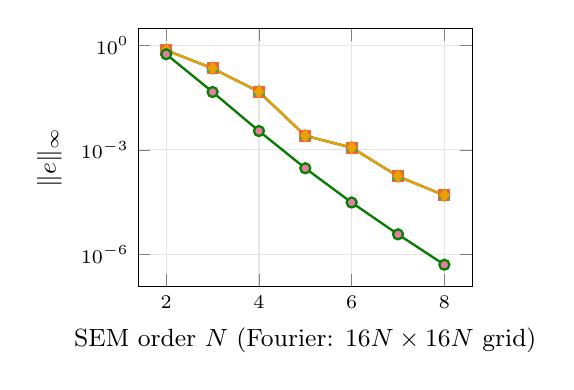
\begin{tikzpicture}
    \begin{axis}[width=0.48\textwidth, height=0.40\textwidth,
                 xlabel={SEM order $N$ (Fourier: $16N\times16N$ grid)}, ylabel={$\|e\|_\infty$},
                 xmode=normal, ymode=log, grid=major, grid style={gray!20},
                 legend style={font=\scriptsize, cells={anchor=west}},
                 tick label style={font=\scriptsize}, label style={font=\small}, legend to name=scleg, legend columns=3]
      \addplot[color=jxsem, mark=*, mark options={solid, fill=jxsem}, solid, thick, mark size=1.8pt] coordinates {(2,0.731752) (3,0.220314) (4,0.0470748) (5,0.00254928) (6,0.00116637) (7,0.000174658) (8,4.95039e-05)};
      \addlegendentry{SEM direct}
      \addplot[color=jxsemamg, mark=square*, mark options={solid, fill=jxsemamg}, solid, thick, mark size=1.8pt] coordinates {(2,0.731752) (3,0.220314) (4,0.0470748) (5,0.00254928) (6,0.00116637) (7,0.000174658) (8,4.95039e-05)};
      \addlegendentry{SEM AMG}
      \addplot[color=jxscdirect, mark=triangle*, mark options={solid, fill=jxscdirect}, solid, thick, mark size=1.8pt] coordinates {(2,0.731752) (3,0.220314) (4,0.0470748) (5,0.00254928) (6,0.00116637) (7,0.000174658) (8,4.95039e-05)};
      \addlegendentry{SC direct}
      \addplot[color=jxscamg, mark=diamond*, mark options={solid, fill=jxscamg}, solid, thick, mark size=1.8pt] coordinates {(2,0.731752) (3,0.220314) (4,0.0470748) (5,0.00254928) (6,0.00116637) (7,0.000174658) (8,4.95039e-05)};
      \addlegendentry{SC AMG}
      \addplot[color=jxps, mark=pentagon*, mark options={solid, fill=jxps}, solid, thick, mark size=1.8pt] coordinates {(2,0.561648) (3,0.0462008) (4,0.0034958) (5,0.000297471) (6,3.08363e-05) (7,3.75822e-06) (8,5.03773e-07)};
      \addlegendentry{pseudo-spectral}
      \addplot[color=jxfft, mark=o, mark options={solid, fill=white}, solid, thick, mark size=1.8pt] coordinates {(2,0.561648) (3,0.0462008) (4,0.0034958) (5,0.000297471) (6,3.08363e-05) (7,3.75822e-06) (8,5.03773e-07)};
      \addlegendentry{FFT}
    \end{axis}
  \end{tikzpicture}
  \hfill
  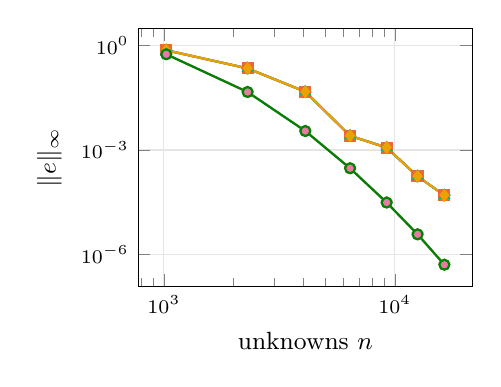
\begin{tikzpicture}
    \begin{axis}[width=0.48\textwidth, height=0.40\textwidth,
                 xlabel={unknowns $n$}, ylabel={$\|e\|_\infty$},
                 xmode=log, ymode=log, grid=major, grid style={gray!20},
                 legend style={font=\scriptsize, cells={anchor=west}},
                 tick label style={font=\scriptsize}, label style={font=\small}]
      \addplot[color=jxsem, mark=*, mark options={solid, fill=jxsem}, solid, thick, mark size=1.8pt] coordinates {(1024,0.731752) (2304,0.220314) (4096,0.0470748) (6400,0.00254928) (9216,0.00116637) (12544,0.000174658) (16384,4.95039e-05)};
      \addplot[color=jxsemamg, mark=square*, mark options={solid, fill=jxsemamg}, solid, thick, mark size=1.8pt] coordinates {(1024,0.731752) (2304,0.220314) (4096,0.0470748) (6400,0.00254928) (9216,0.00116637) (12544,0.000174658) (16384,4.95039e-05)};
      \addplot[color=jxscdirect, mark=triangle*, mark options={solid, fill=jxscdirect}, solid, thick, mark size=1.8pt] coordinates {(1024,0.731752) (2304,0.220314) (4096,0.0470748) (6400,0.00254928) (9216,0.00116637) (12544,0.000174658) (16384,4.95039e-05)};
      \addplot[color=jxscamg, mark=diamond*, mark options={solid, fill=jxscamg}, solid, thick, mark size=1.8pt] coordinates {(1024,0.731752) (2304,0.220314) (4096,0.0470748) (6400,0.00254928) (9216,0.00116637) (12544,0.000174658) (16384,4.95039e-05)};
      \addplot[color=jxps, mark=pentagon*, mark options={solid, fill=jxps}, solid, thick, mark size=1.8pt] coordinates {(1024,0.561648) (2304,0.0462008) (4096,0.0034958) (6400,0.000297471) (9216,3.08363e-05) (12544,3.75822e-06) (16384,5.03773e-07)};
      \addplot[color=jxfft, mark=o, mark options={solid, fill=white}, solid, thick, mark size=1.8pt] coordinates {(1024,0.561648) (2304,0.0462008) (4096,0.0034958) (6400,0.000297471) (9216,3.08363e-05) (12544,3.75822e-06) (16384,5.03773e-07)};
    \end{axis}
  \end{tikzpicture}
  \\[2pt]\ref{scleg}
  \caption{Error against the exact solution versus order (left) and number of unknowns
           (right). The four SEM curves coincide (the same discrete solution), and so do the
           pseudo-spectral and FFT curves.}
  \label{fig:sc-error}
\end{figure}

\begin{figure}[htbp]
  \centering
  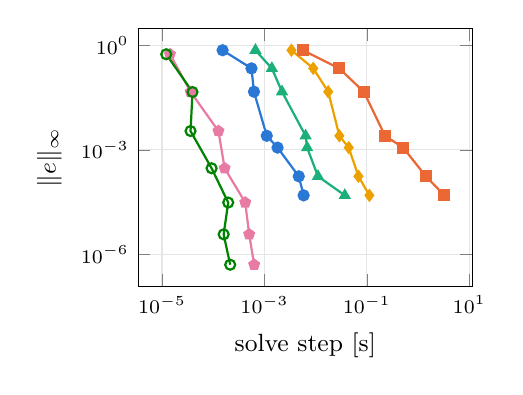
\begin{tikzpicture}
    \begin{axis}[width=0.48\textwidth, height=0.40\textwidth,
                 xlabel={solve step [s]}, ylabel={$\|e\|_\infty$},
                 xmode=log, ymode=log, grid=major, grid style={gray!20},
                 legend style={font=\scriptsize, cells={anchor=west}},
                 tick label style={font=\scriptsize}, label style={font=\small}, legend to name=sclegb, legend columns=3]
      \addplot[color=jxsem, mark=*, mark options={solid, fill=jxsem}, solid, thick, mark size=1.8pt] coordinates {(0.000152431,0.731752) (0.00055852,0.220314) (0.000624552,0.0470748) (0.00111073,0.00254928) (0.00180604,0.00116637) (0.00469084,0.000174658) (0.00583525,4.95039e-05)};
      \addlegendentry{SEM direct}
      \addplot[color=jxsemamg, mark=square*, mark options={solid, fill=jxsemamg}, solid, thick, mark size=1.8pt] coordinates {(0.00565536,0.731752) (0.0288679,0.220314) (0.087398,0.0470748) (0.227232,0.00254928) (0.513428,0.00116637) (1.42727,0.000174658) (3.27811,4.95039e-05)};
      \addlegendentry{SEM AMG}
      \addplot[color=jxscdirect, mark=triangle*, mark options={solid, fill=jxscdirect}, solid, thick, mark size=1.8pt] coordinates {(0.000667467,0.731752) (0.00139912,0.220314) (0.00220466,0.0470748) (0.00637712,0.00254928) (0.00682894,0.00116637) (0.0111215,0.000174658) (0.0372081,4.95039e-05)};
      \addlegendentry{SC direct}
      \addplot[color=jxscamg, mark=diamond*, mark options={solid, fill=jxscamg}, solid, thick, mark size=1.8pt] coordinates {(0.00337714,0.731752) (0.0089975,0.220314) (0.0176314,0.0470748) (0.0291203,0.00254928) (0.0443627,0.00116637) (0.0686788,0.000174658) (0.112363,4.95039e-05)};
      \addlegendentry{SC AMG}
      \addplot[color=jxps, mark=pentagon*, mark options={solid, fill=jxps}, solid, thick, mark size=1.8pt] coordinates {(1.4275e-05,0.561648) (3.6248e-05,0.0462008) (0.000126507,0.0034958) (0.000167133,0.000297471) (0.000422151,3.08363e-05) (0.000503398,3.75822e-06) (0.000630872,5.03773e-07)};
      \addlegendentry{pseudo-spectral}
      \addplot[color=jxfft, mark=o, mark options={solid, fill=white}, solid, thick, mark size=1.8pt] coordinates {(1.2078e-05,0.561648) (3.939e-05,0.0462008) (3.6012e-05,0.0034958) (9.2952e-05,0.000297471) (0.000196288,3.08363e-05) (0.000159729,3.75822e-06) (0.000214428,5.03773e-07)};
      \addlegendentry{FFT}
    \end{axis}
  \end{tikzpicture}
  \hfill
  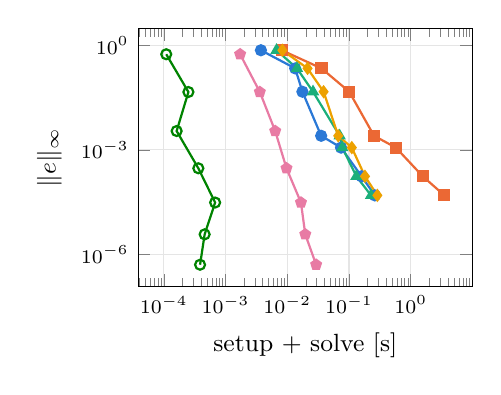
\begin{tikzpicture}
    \begin{axis}[width=0.48\textwidth, height=0.40\textwidth,
                 xlabel={setup + solve [s]}, ylabel={$\|e\|_\infty$},
                 xmode=log, ymode=log, grid=major, grid style={gray!20},
                 legend style={font=\scriptsize, cells={anchor=west}},
                 tick label style={font=\scriptsize}, label style={font=\small}]
      \addplot[color=jxsem, mark=*, mark options={solid, fill=jxsem}, solid, thick, mark size=1.8pt] coordinates {(0.00374215,0.731752) (0.0134391,0.220314) (0.0175939,0.0470748) (0.0354009,0.00254928) (0.0742986,0.00116637) (0.159507,0.000174658) (0.262042,4.95039e-05)};
      \addplot[color=jxsemamg, mark=square*, mark options={solid, fill=jxsemamg}, solid, thick, mark size=1.8pt] coordinates {(0.00812317,0.731752) (0.0358768,0.220314) (0.100848,0.0470748) (0.254248,0.00254928) (0.574367,0.00116637) (1.56588,0.000174658) (3.50514,4.95039e-05)};
      \addplot[color=jxscdirect, mark=triangle*, mark options={solid, fill=jxscdirect}, solid, thick, mark size=1.8pt] coordinates {(0.00669611,0.731752) (0.0143678,0.220314) (0.0261428,0.0470748) (0.0705546,0.00254928) (0.0778576,0.00116637) (0.131578,0.000174658) (0.227487,4.95039e-05)};
      \addplot[color=jxscamg, mark=diamond*, mark options={solid, fill=jxscamg}, solid, thick, mark size=1.8pt] coordinates {(0.00834252,0.731752) (0.0212965,0.220314) (0.0387745,0.0470748) (0.0669096,0.00254928) (0.111024,0.00116637) (0.181313,0.000174658) (0.287995,4.95039e-05)};
      \addplot[color=jxps, mark=pentagon*, mark options={solid, fill=jxps}, solid, thick, mark size=1.8pt] coordinates {(0.00172248,0.561648) (0.00359302,0.0462008) (0.0063751,0.0034958) (0.00971423,0.000297471) (0.0166562,3.08363e-05) (0.0195638,3.75822e-06) (0.0293551,5.03773e-07)};
      \addplot[color=jxfft, mark=o, mark options={solid, fill=white}, solid, thick, mark size=1.8pt] coordinates {(0.000109514,0.561648) (0.000250324,0.0462008) (0.00016137,0.0034958) (0.000362438,0.000297471) (0.000678374,3.08363e-05) (0.000458652,3.75822e-06) (0.000386749,5.03773e-07)};
    \end{axis}
  \end{tikzpicture}
  \\[4pt]
  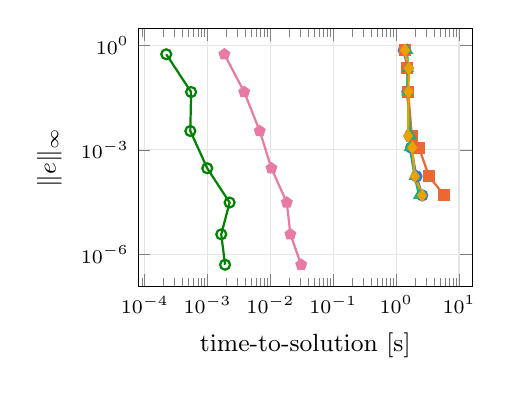
\begin{tikzpicture}
    \begin{axis}[width=0.48\textwidth, height=0.40\textwidth,
                 xlabel={time-to-solution [s]}, ylabel={$\|e\|_\infty$},
                 xmode=log, ymode=log, grid=major, grid style={gray!20},
                 legend style={font=\scriptsize, cells={anchor=west}},
                 tick label style={font=\scriptsize}, label style={font=\small}]
      \addplot[color=jxsem, mark=*, mark options={solid, fill=jxsem}, solid, thick, mark size=1.8pt] coordinates {(1.32432,0.731752) (1.52859,0.220314) (1.51045,0.0470748) (1.65165,0.00254928) (1.72772,0.00116637) (2.1083,0.000174658) (2.60946,4.95039e-05)};
      \addplot[color=jxsemamg, mark=square*, mark options={solid, fill=jxsemamg}, solid, thick, mark size=1.8pt] coordinates {(1.37726,0.731752) (1.50794,0.220314) (1.55535,0.0470748) (1.77967,0.00254928) (2.30925,0.00116637) (3.33863,0.000174658) (5.85828,4.95039e-05)};
      \addplot[color=jxscdirect, mark=triangle*, mark options={solid, fill=jxscdirect}, solid, thick, mark size=1.8pt] coordinates {(1.49708,0.731752) (1.53743,0.220314) (1.50047,0.0470748) (1.71279,0.00254928) (1.64951,0.00116637) (1.97395,0.000174658) (2.31796,4.95039e-05)};
      \addplot[color=jxscamg, mark=diamond*, mark options={solid, fill=jxscamg}, solid, thick, mark size=1.8pt] coordinates {(1.38723,0.731752) (1.59109,0.220314) (1.57513,0.0470748) (1.54663,0.00254928) (1.80604,0.00116637) (1.9908,0.000174658) (2.59874,4.95039e-05)};
      \addplot[color=jxps, mark=pentagon*, mark options={solid, fill=jxps}, solid, thick, mark size=1.8pt] coordinates {(0.00185167,0.561648) (0.00382646,0.0462008) (0.00675892,0.0034958) (0.0103786,0.000297471) (0.0182445,3.08363e-05) (0.0207658,3.75822e-06) (0.0308972,5.03773e-07)};
      \addplot[color=jxfft, mark=o, mark options={solid, fill=white}, solid, thick, mark size=1.8pt] coordinates {(0.000219989,0.561648) (0.000546883,0.0462008) (0.000531499,0.0034958) (0.000988189,0.000297471) (0.00224185,3.08363e-05) (0.0016504,3.75822e-06) (0.00189743,5.03773e-07)};
    \end{axis}
  \end{tikzpicture}
  \hfill
  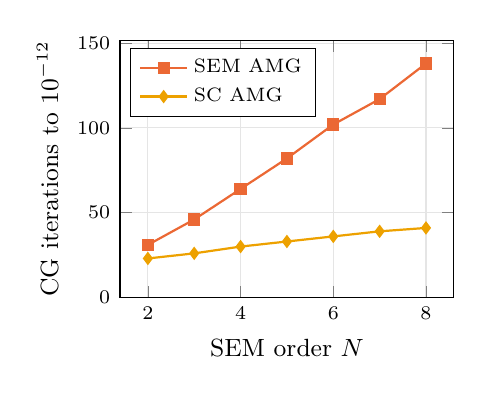
\begin{tikzpicture}
    \begin{axis}[width=0.48\textwidth, height=0.40\textwidth,
                 xlabel={SEM order $N$}, ylabel={CG iterations to $10^{-12}$},
                 xmode=normal, ymode=normal, grid=major, grid style={gray!20},
                 legend style={font=\scriptsize, cells={anchor=west}},
                 tick label style={font=\scriptsize}, label style={font=\small}, ymin=0, legend pos=north west]
      \addplot[color=jxsemamg, mark=square*, mark options={solid, fill=jxsemamg}, solid, thick, mark size=1.8pt] coordinates {(2,31) (3,46) (4,64) (5,82) (6,102) (7,117) (8,138)};
      \addlegendentry{SEM AMG}
      \addplot[color=jxscamg, mark=diamond*, mark options={solid, fill=jxscamg}, solid, thick, mark size=1.8pt] coordinates {(2,23) (3,26) (4,30) (5,33) (6,36) (7,39) (8,41)};
      \addlegendentry{SC AMG}
    \end{axis}
  \end{tikzpicture}
  \\[2pt]\ref{sclegb}
  \caption{Second-run wall-clock. Top: error versus the solve step alone (left) and versus
           the solver cost, setup plus solve (right). Bottom left: error versus the
           time-to-solution including all infrastructure; each curve runs over
           $N=2,\dots,8$. Bottom right: iterations of AMG-preconditioned CG on the full
           SEM system and on the statically condensed skeleton system.}
  \label{fig:sc-time}
\end{figure}

\paragraph{Findings.}
\begin{enumerate}
  \item \textbf{One discrete solution, four solves.} SEM direct, SEM AMG, SC direct and SC
        AMG return the same solution: the errors of SC direct and SEM direct differ by at
        most $4.9\times10^{-13}$, those of the AMG solves by amounts consistent with the CG
        tolerance. The SEM error falls exponentially with the order, from
        $7.3\times10^{-1}$ at $N=2$ to $5.0\times10^{-5}$ at $N=8$
        (Table~\ref{tab:sc-accuracy}).
  \item \textbf{Static condensation makes AMG far more effective.} On the full SEM system
        the CG iterations grow from 31 to 138 between $N=2$ and
        $N=8$: smoothed aggregation, designed for low-order stencils, degrades as the
        element-interior modes of the high-order discretisation are added. On the
        skeleton system they grow only from 23 to 41
        (Figure~\ref{fig:sc-time}, bottom right), and each iteration is cheaper because
        the system is 4.3$\times$ smaller. At $N=8$ the SC AMG solve step is
        29$\times$ faster than AMG on the full system.
  \item \textbf{The direct triangular solves are the fastest solve step; condensation makes
        the setup cheap.} A Cholesky back-solve of the $16\,384$-unknown system takes
        5.84\,ms, 19$\times$ less than the SC AMG solve step
        (Table~\ref{tab:sc-solve}). Setup changes the ranking (Table~\ref{tab:sc-cost}): at
        $N=8$ the solver cost is 227\,ms for SC direct,
        288\,ms for SC AMG, 262\,ms for SEM direct and
        3.51\,s for SEM AMG. After static condensation both skeleton
        solves are as cheap as the direct solve of the full system, while AMG on the full
        system is not competitive. Over this range the Cholesky factorisation of the full
        system grows as $n^{1.56}$, as expected ($n^{3/2}$) for nested-dissection
        orderings in two dimensions.
  \item \textbf{The SEM infrastructure dominates the time-to-solution} of SEM direct,
        SC direct and SC AMG: reading the mesh and building the high-order nodes, the
        metric terms and the matrices takes 1.3--2.4\,s, against at most
        288\,ms for the cost of these three solvers, so their
        times-to-solution differ by at most a factor of 1.13
        (Table~\ref{tab:sc-total}). SEM AMG is the exception: its cost grows to
        3.51\,s at $N=8$, and its time-to-solution there is
        2.2$\times$ that of SEM direct.
  \item \textbf{Spectral baselines.} The pseudo-spectral and FFT solvers compute the same
        Fourier solution: their errors agree to 6 digits. Their error falls
        geometrically with the grid, from $5.6\times10^{-1}$ on the
        $32^2$ grid to $5.0\times10^{-7}$ on the $128^2$ grid, consistent with
        the $r^{N_g/2}$ decay of the Fourier coefficients of \eqref{eq:sc-exact}. At
        the same number of unknowns it is 98$\times$ smaller than the SEM
        error at $N=8$. The analytic, periodic solution suits a global Fourier basis,
        which converges geometrically in $N_g$, while the SEM gains its accuracy element by
        element. Their time-to-solution at the largest size is 30.9\,ms and 1.9\,ms.
\end{enumerate}

\paragraph{Implementation notes.} The timings were obtained after two performance
defects in the element-learning code had been removed, neither of which changes any
result: the arrays of the element-learning data structure are declared with concrete
types (untyped fields made every access in the condensation loops dynamically
dispatched), and the correction $\sum_e A_{b,o_e}T^e$ in \eqref{eq:sc-schur} is
assembled from (row, column, value) triplets by a single sparse-matrix construction
instead of by insertions into a compressed sparse matrix, whose cost grows
quadratically with the number of entries. Together they reduced the condensation step
at $N=8$ from 2.9\,s to about 0.05\,s.

\subsection{When can AMG beat the direct solve? Recommended experiments}
\label{sec:sc-recommendations}
The benchmark above is small ($n\le16\,384$), two-dimensional, run on a single node,
and has one right-hand side and a constant coefficient: all conditions that favour a
sparse direct solver. The following experiments are designed to locate the settings,
if any, in which AMG on the SEM system --- full or condensed --- wins.

\begin{enumerate}
  \item \textbf{Refine the mesh at fixed order ($h$-refinement).} Our sweep varies the order
        on a fixed mesh, which mixes two effects: the size of the system and the
        high-order character that degrades AMG. At fixed $N\in\{2,4,8\}$, refine the mesh
        through $16^2,32^2,\dots,256^2$ elements (up to $\sim4\times10^6$ unknowns at
        $N=8$). A scalable AMG keeps the iteration count nearly constant, so its cost grows
        like $n$, whereas the Cholesky factorisation grows like $n^{3/2}$ in time and
        $n\log n$ in memory in 2D. \emph{Rough extrapolation, to be verified:} if the AMG
        iteration counts stay constant and the direct cost keeps growing like
        $n^{1.56}$, the solver costs measured at $n=16\,384$ and $N=8$
        put the crossover with the full direct solve near $n\approx 2\times10^{4}$ for SC AMG and
        near $n\approx 2\times10^{6}$ for AMG on the full system. Both assumptions
        must be checked: the iteration counts of aggregation AMG on high-order matrices
        usually grow slowly under refinement, and the factorisation exponent depends on
        the ordering. Report where, and whether, the curves cross.
  \item \textbf{Go to three dimensions.} Nested-dissection fill is much larger in 3D
        ($O(n^2)$ time, $O(n^{4/3})$ memory) and the SEM element blocks are denser
        ($(N+1)^3$ couplings). This is the most likely setting for AMG, and for the
        condensed system in particular, to win, often already at $\sim10^5$ unknowns;
        memory, not time, is usually what stops the direct solver first.
  \item \textbf{Match the stopping tolerance to the discretisation error.} A relative
        residual of $10^{-12}$ is far below the discretisation error at low order
        ($\|e\|_\infty\approx 7.3\times10^{-1}$ at $N=2$). Stop CG when the algebraic
        error is a fixed fraction (e.g.\ $0.1$) of the discretisation error and report
        iterations and time against $N$; the direct solver cannot exploit this, AMG can.
  \item \textbf{Use a preconditioner designed for high order.} The iteration growth on the
        full system comes from applying an aggregation AMG built for low-order stencils
        directly to the high-order matrix. Standard remedies to test: (i) AMG on the
        low-order finite-element matrix assembled on the same Gauss--Lobatto nodes, which
        is spectrally equivalent to the SEM matrix and much sparser (9 entries per row
        instead of up to $(2N+1)^2$), as the preconditioner of CG on the SEM system;
        (ii) $p$-multigrid (coarsening in the order down to $N=1$, then AMG); (iii) the
        AMG settings: Ruge--St\"uben coarsening, strength threshold, smoother
        (Gauss--Seidel, Chebyshev, $\ell_1$-Jacobi) and number of smoothing steps. Combine
        each with static condensation.
  \item \textbf{Amortise over many solves.} In time-dependent or parameter-sweep use
        (implicit diffusion, Helmholtz steps, Newton linearisations, element-learning
        training data) the same matrix serves many right-hand sides. A factorisation is
        then reused as well, which favours the direct solve --- unless the matrix changes
        at every step (variable coefficients, adaptivity), in which case building an AMG
        hierarchy is cheaper than refactorising. Measure setup and solve separately, as
        here, and report the break-even number of right-hand sides.
  \item \textbf{Scale out.} Sparse direct solvers scale poorly in distributed memory, while
        Krylov methods preconditioned by AMG are the standard for large parallel elliptic
        solves. Repeat the $h$-refinement study with MPI (strong and weak scaling), with a
        distributed direct solver (e.g.\ MUMPS) as the baseline.
  \item \textbf{Harder operators.} Deformed or curved elements, variable or anisotropic
        coefficients (the element-learning test cases) and Dirichlet data change the
        conditioning seen by AMG but hardly the cost of a direct solve; repeat the
        comparison on those cases.
  \item \textbf{Measure memory.} Record the peak memory of every solver; in large 2D and in
        3D problems the fill-in of the factorisation is often the binding limit.
  \item \textbf{Report robust timings.} Keep the second-run protocol but repeat each
        measurement several times and report the median (single-shot timings of
        sub-millisecond solves are noisy), fix the numbers of Julia and BLAS threads, and
        state the machine.
\end{enumerate}
